% LDhybrid v1.0 -- A&A manuscript draft (A&A LaTeX macro package; see AA_CLASS.md).
% Numbers come from studies/*/results.md. Citations marked % VERIFY need their
% volume/page checked on ADS. Compile: tectonic ldhybrid.tex
\documentclass{aa}

\usepackage{graphicx}
\usepackage{txfonts}
\usepackage{amsmath}
\usepackage[colorlinks=true,linkcolor=black,citecolor=black,urlcolor=black]{hyperref}

\newcommand{\ppm}{\,\textrm{ppm}}
\newcommand{\teff}{T_{\rm eff}}

\begin{document}

\title{Limb-darkening coefficients for rational laws with elementary transit
light curves\thanks{The tables described in Table~\ref{tab:cds} are only
available in electronic form at the CDS via anonymous ftp to
\url{cdsarc.cds.unistra.fr} (130.79.128.5) or via
\url{https://cdsarc.cds.unistra.fr/viz-bin/cat/J/A+A/}}}
\subtitle{PHOENIX, MPS-ATLAS, and ATLAS models for exoplanet passbands}

\author{$\langle$Author list$\rangle$\inst{1}}

\institute{$\langle$Institution$\rangle$\\
\email{$\langle$email$\rangle$}}

\date{Received $\langle$date$\rangle$ / Accepted $\langle$date$\rangle$}

\abstract
{Rational limb-darkening laws, polynomials in $\mu^2$ plus double poles
$(\mu^2+\varepsilon)^{-2}$ beyond the stellar limb, give transit light curves in
closed, elementary form for planets of any elliptical outline, which the
standard laws do not.}
{We provide theoretical coefficients for three such laws, hybrid2, hybrid4, and
hybrid5, for the passbands used in transit observations, in the manner of the
tables of Claret and collaborators.}
{We integrated the specific intensities of spherical PHOENIX-ACES models and of
plane-parallel MPS-ATLAS (two sets) and ATLAS9 models over 38 passbands with
photon weighting, placed the limb of spherical models at the maximum intensity
gradient, and fitted the laws by least squares uniform in projected radius,
constrained to positive and monotonic profiles. Quadratic, power-2, and
four-term coefficients were computed in the same way. We also tabulate
three-dimensional and magnetic corrections from MURaM and Stagger models.}
{Fitting uniformly in radius rather than in $\mu$ reduces the light-curve error
of the fitted laws by factors of 3--10. The hybrid5 law reproduces the model
light curves to a median of 2.7\ppm{} (PHOENIX) and 0.95\ppm{} (MPS-ATLAS),
better than the four-term law, and the observed solar limb darkening to
3--5\ppm. Every hybrid coefficient set is physical. Against Kepler and TESS
measurements, the MPS-ATLAS predictions show the known offset, which a 100\,G
MURaM correction removes; against JWST it removes about a third.}
{The coefficients, coefficient spectra for arbitrary bandpasses, and an
interpolation code are made available.}

\keywords{stars: atmospheres -- planets and satellites: general --
techniques: photometric -- methods: numerical}

\maketitle

%======================================================================
\section{Introduction}
%======================================================================
Theoretical limb-darkening coefficients are a standard ingredient of transit
and eclipse modelling. Since \citet{claret2000} introduced the four-term law and
fitted it across the ATLAS grid, tables of coefficients for successive laws,
model atmospheres, and passbands have followed
\citep{claretbloemen2011,claret2012,claret2013,claret2017,claret2018,claretsouthworth2022,claretsouthworth2023,claret2025}.
The choice of law has so far been driven by accuracy: the four-term law
represents model intensities best, and the power-2 law \citep{hestroffer1997}
is the most accurate two-parameter law \citep{maxted2018,claretsouthworth2022}.

A second consideration is computability. For a circular planet every standard
law has a closed-form light curve \citep{mandelagol2002,agol2020}. For a planet
of elliptical outline, the projection of an oblate or rotating planet, only laws
whose intensity is a polynomial in $\mu^2$ plus terms with poles of order two or
more beyond the limb give elementary light curves; odd powers of $\mu$ lead to
elliptic integrals and fractional powers to no closed form at all
\citep{squishier}. Adding double poles to the even polynomial restores the steep
limb that the polynomial alone cannot follow, and the resulting ``hybrid'' laws
rival the four-term law in accuracy \citep{squishier}.

This paper provides, for these laws, what Claret's papers provide for the
standard ones: coefficients for a broad range of stellar parameters and for the
passbands of transit work, with quantified fit quality. Section~\ref{sec:laws}
defines the laws, Sect.~\ref{sec:models} the models and passbands,
Sect.~\ref{sec:method} the fitting method, Sect.~\ref{sec:quality} the quality
of the fits, Sect.~\ref{sec:obs} comparisons with observations, and
Sect.~\ref{sec:tables} the tables.

%======================================================================
\section{The laws}\label{sec:laws}
%======================================================================
All laws are written as
\begin{equation}
\frac{I(\mu)}{I(1)}=1-\sum_j w_j\,T_j(\mu),
\end{equation}
where each shape $T_j$ equals 1 at the limb and 0 at the centre, so that $w_j$
is the fraction of the centre-to-limb drop carried by term $j$ and
$I(0)/I(1)=1-\sum_j w_j$. With the normalised pole term
\begin{equation}
\Pi_\varepsilon(\mu)=\frac{(\mu^2+\varepsilon)^{-2}-(1+\varepsilon)^{-2}}{\varepsilon^{-2}-(1+\varepsilon)^{-2}},
\end{equation}
the three laws are
\begin{align}
\text{hybrid2:}\ & T=\{1-\mu^2,\ \Pi_{0.36}\},\\
\text{hybrid4:}\ & T=\{1-\mu^4,\ (1-\mu^2)^2,\ \Pi_{\varepsilon_0},\ \Pi_{\varepsilon_1}\},\\
\text{hybrid5:}\ & T=\{1-\mu^4,\ (1-\mu^2)^2,\ \Pi_{\varepsilon_0},\ \Pi_{\varepsilon_1},\ \Pi_{\varepsilon_2}\},
\end{align}
with poles on the analytic ladder
$\varepsilon_k=\exp[2\pi(\sqrt{k+1/2}-\sqrt K)]$ for $K=2$
($\varepsilon=0.011762$, 0.30408) and $K=3$ (0.0015966, 0.041275, 0.38743),
derived by \citet{squishier} from an exact double-pole representation of
$\mu^{2\alpha}$. The single pole of hybrid2 has no analytic placement; we tuned
it on 7524 model--passband combinations (Sect.~\ref{sec:method}), which moved
it from the value 0.208 tuned on J-band PHOENIX profiles by \citet{squishier}
to $\varepsilon=0.36$. All pole positions are fixed constants, so the laws are
linear in their weights.

Linearity has three consequences used below. Firstly, positivity and
monotonicity are linear inequalities in $w$, so the physical region is convex
and a constrained fit is a convex quadratic programme with a unique optimum. For
hybrid2 this region is exactly a triangle; for hybrid4 and hybrid5 the simplex
$w_j\ge0$, $\sum w_j\le1$ is a sufficient region that contains every model fit
in this work. Secondly, linear interpolation of tabulated weights between
models stays inside the physical region. Thirdly, a least-squares fit is a fixed
linear map of the intensity data, so per-wavelength coefficients integrate
exactly to band coefficients (Sect.~\ref{sec:spectra}). The sampling coordinates
$q\in[0,1]^n$ of \citet{squishier}, which map the triangle and the simplex to
the unit hypercube in the manner of \citet{kipping2013}, are provided with the
code.

%======================================================================
\section{Model atmospheres and passbands}\label{sec:models}
%======================================================================
We used three 1D grids, restricted to dwarfs and subgiants
($2300\le\teff\le7400$\,K, $3.5\le\log g\le5.5$, $-2\le[{\rm M/H}]\le+1$):
PHOENIX-ACES-AGSS-COND SpecInt v3.0 \citep{husser2013}, spherical, with 78
$\mu$ points and 1\,\AA{} sampling to 5.5\,$\mu$m (1682 models); MPS-ATLAS
\citep{witzke2021,kostogryz2022} Set~1 and Set~2, which differ in abundances and
mixing-length treatment, plane-parallel with 24 $\mu$ points and ODF wavelength
sampling (16\,974 models each); and ATLAS9 (the subset distributed with
ExoTiC-LD; \citealt{grant2024}), used only for JWST/MIRI LRS (5--14\,$\mu$m),
which lies beyond the PHOENIX data, for 3500--6500\,K.

Intensities were integrated over each passband with photon weighting,
$I_{\rm b}(\mu)\propto\int I_\lambda(\mu)\,\lambda\,S(\lambda)\,{\rm d}\lambda$,
using exact integrals over contiguous wavelength bins (the PHOENIX spectra were
reduced to $R=3000$ photon bins, with a reduction error below
$1.2\times10^{-5}$ in $I/I(1)$).

The 38 passbands are Kepler, TESS, CHEOPS, NGTS, Spitzer/IRAC 1 and 2 (subarray
and full array), Johnson $BV$, Cousins $RI$, Sloan $g'r'i'z'$, 2MASS
$JHK_{\rm s}$, HST WFC3 (G102, G141, and UVIS G280 $\pm1$) and STIS (G430L,
G750L), and JWST NIRISS/SOSS orders 1 and 2, NIRSpec PRISM, G140M/H, G235M/H,
and G395M/H, NIRCam F322W2 and F444W, and MIRI LRS. Photometric curves are from
the SVO Filter Profile Service, IRAC curves from the Spitzer Science Center, and
HST and JWST modes from \citet{grant2024}. Each curve is used as a
photon-counting response except the Bessell Johnson--Cousins curves; the
energy-counter flag in the SVO record for TESS would otherwise shift TESS
profiles by $\sim$1\%.

%======================================================================
\section{Method}\label{sec:method}
%======================================================================
\subsection{The limb of spherical models}
In spherical models $\mu$ is measured from the outermost model shell, outside
the photosphere. Following \citet{espinoza2015} and
\citet{claret2017,claretsouthworth2023}, we placed the stellar edge $r_{\rm c}$
at the node of maximum $|{\rm d}I/{\rm d}r|$ (method M1 of
\citealt{claretsouthworth2023}), discarded the outer points, and rescaled
$\mu'=\sqrt{1-(r/r_{\rm c})^2}$. We tabulate $\mu_{\rm cri}=\sqrt{1-r_{\rm c}^2}$;
our values agree with those of \citet{claretsouthworth2023} to $\sim10^{-3}$.

\subsection{Fitting}
The laws were fitted to $I(\mu)/I(1)$, with $I(1)=1$ fixed, by least squares on
a 2000-point resample of the profile (monotone cubic interpolation) uniform in
projected radius $r=\sqrt{1-\mu^2}$, subject to the physical constraints.
Claret's least-squares method weights points uniformly in $\mu$, which gives the
outer 0.5\% of the radius ($\mu<0.1$) a tenth of the weight, whereas a transit
samples the disc by area. Table~\ref{tab:weighting} compares the weightings by
the quantity a user cares about, the error of the light curve: fitting uniformly
in $r$ (or, equivalently within the noise, in area) reduces it by factors of
3--10 for every law, consistent with the ``weighted-r'' recipe of
\citet{morello2020}. Constraining to the physical region costs nothing: in our
method study no constraint was active for 400 model--passband combinations, and
over the full grids they are active in at most 1\% of hybrid fits. Imposing flux
conservation \citep{claretbloemen2011} changed the light-curve error by less than
0.5\ppm{} and was not adopted. Quadratic and four-term fits use the same
weighting and their exact positive--monotonic regions; power-2 was fitted
without constraints by the Levenberg--Marquardt method. Fits uniform in $\mu$ are
also tabulated, for comparison with earlier tables.

\begin{table}
\caption{Light-curve error (ppm) of profile fits by weighting, median / worst
over the PHOENIX method-study subset (34 models $\times$ 8 passbands; planet
radius 0.03--0.15, impact parameter 0--0.9).}
\label{tab:weighting}
\centering
\begin{tabular}{lccc}
\hline\hline
Weighting & hybrid5 & Four-term & Power-2\\
\hline
Equal per native node & 43 / 333 & 75 / 204 & 247 / 582\\
Uniform in $\mu$ & 13 / 33 & 55 / 123 & 57 / 152\\
Uniform in $r$ & 4.9 / 11 & 13 / 33 & 22 / 72\\
Uniform in area & 3.9 / 11 & 12 / 31 & 19 / 75\\
\hline
\end{tabular}
\end{table}

\subsection{Light-curve error}
As a measure of fit quality we computed, besides the weighted rms residual
$\sigma$ (Claret's merit function), the largest difference between the transit
light curve of the fitted law and the exact light curve of the tabulated model
profile, for a planet of radius $p=0.1$ at impact parameters 0, 0.3, 0.6, and
0.9. The light curves are computed by Gauss--Legendre quadrature with endpoint
substitutions, accurate to $10^{-8}$\ppm{} against the closed-form hybrid
solution.

\subsection{Sensitivity to the limb}
Because the innermost pole of hybrid5 acts at $\mu\lesssim0.04$, we tested the
choices made at the limb: M1 against M2, one edge per model against one per
passband, and resampling the profile on the coarser $\mu$ grids of ATLAS,
MPS-ATLAS, and Stagger. Each changes the fitted light curves by a median of
$\lesssim5\ppm$ (90th percentile $\lesssim8\ppm$), whereas PHOENIX and MPS-ATLAS
for the same star differ by a median of 170\ppm. The light curves of hybrid5
are the least sensitive of all laws, but its innermost-pole weight $w_3$ is
weakly determined: limb choices move it by 0.03--0.10 at almost no cost in
light-curve terms (Fig.~\ref{fig:coef}).

%======================================================================
\section{Quality of the fits}\label{sec:quality}
%======================================================================
Figure~\ref{fig:profiles} shows two profiles and the residuals of the fitted
laws, and Fig.~\ref{fig:quality} the light-curve error against $\teff$. Over all
models and passbands (Table~\ref{tab:quality}) hybrid5 is the most accurate law
on both grids, hybrid4 is comparable to the four-term law on PHOENIX but weaker
on MPS-ATLAS, and hybrid2 matches the quadratic law in median and improves on it
in the tails. Power-2 remains the best two-parameter law, but it is not
elementary for an ellipse and is unphysical ($c>1$) in 8.6\% of PHOENIX rows.
All hybrid rows are physical. The worst hybrid5 rows (56 of 63\,916 above
15\ppm) are metal-poor models at 2300--2500\,K in blue passbands, where the
PHOENIX profile itself brightens towards the limb at $\mu\approx0.01$--0.02 and
the monotonicity constraint becomes active.

\begin{table*}
\caption{Light-curve error (ppm) of the tabulated fits: median / 99th
percentile / maximum over all models and passbands.}
\label{tab:quality}
\centering
\begin{tabular}{lccc}
\hline\hline
Law & PHOENIX & MPS-ATLAS Set 2 & ATLAS9 (MIRI LRS)\\
\hline
hybrid5 & 2.7 / 6.3 / 50 & 0.95 / 4.3 / 7.2 & 1.4 / 2.1 / 2.2\\
hybrid4 & 3.8 / 16 / 61 & 6.8 / 14 / 18 & 1.7 / 2.8 / 7.1\\
Four-term & 8.0 / 19 / 75 & 1.4 / 5.8 / 10 & 2.3 / 3.2 / 3.4\\
Power-2 & 16 / 62 / 188 & 7.2 / 34 / 122 & 4.2 / 7.0 / 7.9\\
hybrid2 & 44 / 114 / 344 & 43 / 83 / 110 & 19 / 31 / 51\\
Quadratic & 44 / 134 / 508 & 51 / 100 / 131 & 22 / 36 / 58\\
\hline
\end{tabular}
\end{table*}

\begin{figure*}
\centering
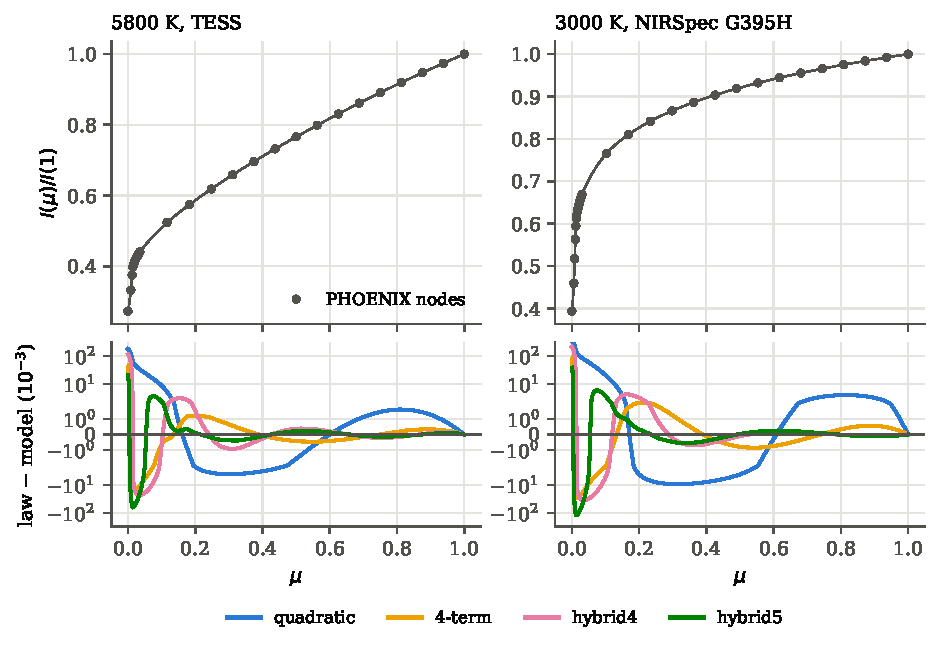
\includegraphics[width=17cm]{figures/fig_profiles.pdf}
\caption{Band-integrated PHOENIX profiles after the limb cut, with the fitted
laws (top; inset: the limb), and the residuals of the fits on a symmetric
logarithmic scale (bottom).}
\label{fig:profiles}
\end{figure*}

\begin{figure*}
\centering
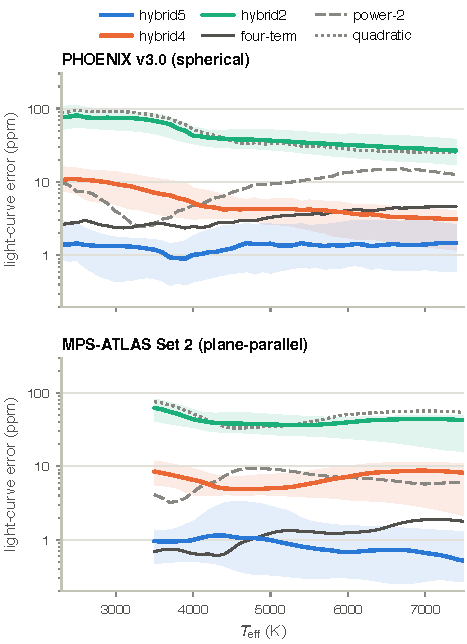
\includegraphics[width=17cm]{figures/fig_quality.pdf}
\caption{Light-curve error of the tabulated fits against $\teff$: median over
passbands, gravities, and metallicities (lines) and 16th--84th percentiles for
the hybrid laws (bands).}
\label{fig:quality}
\end{figure*}

\begin{figure*}
\centering
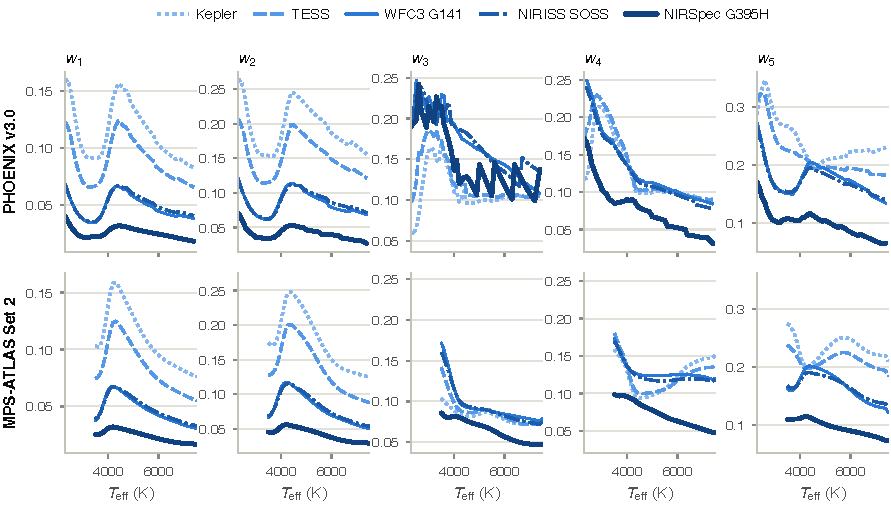
\includegraphics[width=17cm]{figures/fig_coefficients.pdf}
\caption{hybrid5 weights against $\teff$ for $\log g=4.5$ and $[{\rm M/H}]=0$
in five passbands. The innermost-pole weight $w_3$ is weakly determined
(Sect.~\ref{sec:method}).}
\label{fig:coef}
\end{figure*}

The tabulated fits can be interpolated with little loss: interpolating linearly
between grid points, tested by leaving out a model, changes the light curve by a
median of 5\ppm{} in $\teff$ (200\,K gap), 15\ppm{} in $\log g$, and 13\ppm{} in
[M/H] (1\,dex gaps). The coefficients of PHOENIX and of the two MPS-ATLAS sets
for the same star differ by a median of 93\ppm{} (90th percentile 285\ppm) in
light-curve terms. This model systematic, which we tabulate, dominates every
fitting choice.

%======================================================================
\section{Comparison with observations}\label{sec:obs}
%======================================================================
\subsection{The Sun}
Fitted directly to the continuum centre-to-limb profiles of \citet{neckel1994} at
30 wavelengths (303--1099\,nm), hybrid5 reproduces their light curves to a median
of 3--5\ppm{} (four-term 4--6, power-2 7--24, quadratic 21--47\ppm). Among the
models, MPS-ATLAS Set~1 (optical, median 25\ppm) and MURaM with a small-scale
dynamo (near-infrared, 23\ppm) are closest to the observed Sun; PHOENIX v3.0 is
furthest (156--307\ppm).

\subsection{Kepler and TESS}
Figure~\ref{fig:valid} compares the predicted $h'_1=I(2/3)$ and
$h'_2=I(2/3)-I(1/3)$ with the measurements of \citet{maxted2023}. Our four-term
predictions from the MPS-ATLAS spectra reproduce his published offsets for these
models within $1\sigma$, and hybrid5 gives the same offsets: they belong to the
models, not to the law. Adding the MURaM 100\,G correction of
\citet{kostogryz2026} to MPS-ATLAS Set~2 removes them (Kepler:
$\Delta h'_1=-0.002\pm0.002$, $\Delta h'_2=-0.004\pm0.003$), as found by
\citet{kostogryz2024}. The TESS quadratic coefficients of \citet{patel2022} are
reproduced by our PHOENIX values to 0.01 when computed in the same way
\citep[SPAM;][]{howarth2011}, but they are too noisy and degenerate to
discriminate further.

\subsection{JWST}
Against the per-wavelength limb intensities $\ell$ of \citet{sing2026} for six
FGK hosts, the MPS-ATLAS predictions are too dark at the limb by
$\Delta\ell=+0.035\pm0.031$ (star-to-star scatter), in agreement with their
result; the 100\,G correction reduces this to $+0.024$. With the geometric
r-method rescaling used here, PHOENIX shows a similar offset ($+0.041$); the
smaller PHOENIX offset found by \citet{sing2026} follows from their linear
rescaling of $\mu$, which moves $\ell$ by $\approx0.03$.

\begin{figure*}
\centering
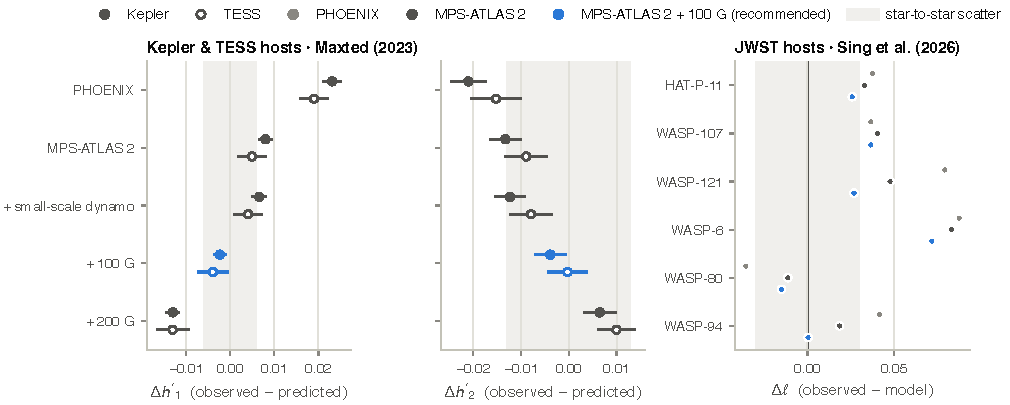
\includegraphics[width=17cm]{figures/fig_validation.pdf}
\caption{Offsets of hybrid5 predictions from measured limb darkening. Left:
Kepler and TESS hosts with $b<0.65$ \citep{maxted2023}, without and with MURaM
corrections. Right: JWST hosts \citep{sing2026}, per star. Shading marks the
star-to-star scatter.}
\label{fig:valid}
\end{figure*}

%======================================================================
\section{The tables}\label{sec:tables}
%======================================================================
The coefficients are given in 24 tables at the CDS, one per grid and law
(Table~\ref{tab:cds}). Each record contains, for one model, passband, and
fitting method ($r$ or $\mu$), $\teff$, $\log g$, [M/H], the passband, the
method, $\mu_{\rm cri}$, the coefficients, the weighted rms residual $\sigma$,
the largest intensity residual, the relative flux error, the light-curve error,
and flags for physicality and for an active constraint.

\begin{table*}
\caption{Tables available at the CDS. Each grid has one file
\texttt{<grid>\_<law>.dat} for each law (hybrid2, hybrid4, hybrid5, quadratic,
four-term \texttt{claret4}, and power-2 \texttt{power2}).}
\label{tab:cds}
\centering
\begin{tabular}{llllllr}
\hline\hline
Grid & Models & $\teff$ (K) & $\log g$ & [M/H] & Passbands & Records per file\\
\hline
\texttt{phoenix} & PHOENIX-ACES v3.0, spherical & 2300--7400 & 3.5--5.5 & $-2.0$ to $+1.0$ (7) & 38 & 127\,832\\
\texttt{mps1} & MPS-ATLAS Set 1, plane-parallel & 3500--7500 & 3.5--5.0 & $-2.0$ to $+1.0$ (46) & 38 & 1\,290\,024\\
\texttt{mps2} & MPS-ATLAS Set 2, plane-parallel & 3500--7500 & 3.5--5.0 & $-2.0$ to $+1.0$ (46) & 38 & 1\,290\,024\\
\texttt{kurucz} & ATLAS9, plane-parallel & 3500--6500 & 4.0--5.0 & $-2.0$ to $+1.0$ (13) & MIRI LRS & 1\,014\\
\hline
\end{tabular}
\tablefoot{The number of metallicities is given in parentheses. Records cover
both fitting methods, uniform in $r$ (recommended) and uniform in $\mu$.}
\end{table*}

\subsection{Coefficient spectra}\label{sec:spectra}
For PHOENIX we also give, per model, the coefficients of hybrid2, hybrid4, and
hybrid5 in each $R=3000$ bin over 0.1--5.5\,$\mu$m, fitted to the unnormalised
intensity with one stellar edge per model. For any bandpass with bin-averaged
throughput $\bar S_k$, $w_j=\sum_k\bar S_k a_{kj}/\sum_k\bar S_k I_k(1)$
reproduces the direct fit to $10^{-9}$, so coefficients for any spectroscopic
bin follow by summation. They differ from the passband tables by 2--10\ppm{} in
light-curve terms.

\subsection{Corrections, offsets, and interpolation}
We tabulate weight shifts $\Delta w$ for surface magnetic fields (MURaM:
small-scale dynamo, 100, 200, and 300\,G; \citealt{kostogryz2026}) and for 3D
convection (MURaM hydrodynamic and Stagger, \citealt{magic2015}, relative to the
matching 1D models), and the empirical offsets of Sect.~\ref{sec:obs} with their
star-to-star scatter as prior widths. For FGK stars we recommend MPS-ATLAS Set~2
with the 100\,G correction. A self-contained interpolation code (Python, numpy
and scipy only) reads the CDS tables and returns coefficients for given
$(\teff,\log g,[{\rm M/H}])$, interpolating linearly within one grid, which
keeps the hybrid coefficients physical.

%======================================================================
\section{Conclusions}
%======================================================================
We have tabulated coefficients of the rational hybrid limb-darkening laws,
whose transit light curves are elementary for planets of any elliptical outline,
for PHOENIX, MPS-ATLAS, and ATLAS9 models and 38 exoplanet passbands. Weighting
the fits uniformly in projected radius rather than in $\mu$ reduces the
light-curve error of every law by factors of 3--10. hybrid5 is the most accurate
law tested, all hybrid coefficients are physical by construction, and linear
interpolation preserves this. The coefficients inherit the offsets of the model
atmospheres from observed limb darkening, which surface magnetic fields account
for in Kepler and TESS but only partly for JWST.

\begin{acknowledgements}
$\langle$Acknowledgements$\rangle$. This work used the SVO Filter Profile
Service, the VizieR catalogue access tool (CDS, Strasbourg), and the ExoTiC-LD
data bundle.
\end{acknowledgements}

\bibliographystyle{aa}
\begin{thebibliography}{}
\bibitem[{Agol} et~al.(2020)]{agol2020} Agol, E., Luger, R., \& Foreman-Mackey, D. 2020, AJ, 159, 123
\bibitem[{Claret}(2000)]{claret2000} Claret, A. 2000, A\&A, 363, 1081
\bibitem[{Claret}(2017)]{claret2017} Claret, A. 2017, A\&A, 600, A30
\bibitem[{Claret}(2018)]{claret2018} Claret, A. 2018, A\&A, 618, A20
\bibitem[{Claret} \& {Bloemen}(2011)]{claretbloemen2011} Claret, A., \& Bloemen, S. 2011, A\&A, 529, A75
\bibitem[{Claret} et~al.(2012)]{claret2012} Claret, A., Hauschildt, P. H., \& Witte, S. 2012, A\&A, 546, A14
\bibitem[{Claret} et~al.(2013)]{claret2013} Claret, A., Hauschildt, P. H., \& Witte, S. 2013, A\&A, 552, A16
\bibitem[{Claret} et~al.(2025)]{claret2025} Claret, A., Hauschildt, P. H., \& Torres, G. 2025, A\&A, 699, A97
\bibitem[{Claret} \& {Southworth}(2022)]{claretsouthworth2022} Claret, A., \& Southworth, J. 2022, A\&A, 664, A128
\bibitem[{Claret} \& {Southworth}(2023)]{claretsouthworth2023} Claret, A., \& Southworth, J. 2023, A\&A, 674, A63
\bibitem[{Espinoza} \& {Jord{\'a}n}(2015)]{espinoza2015} Espinoza, N., \& Jord{\'a}n, A. 2015, MNRAS, 450, 1879
\bibitem[{Grant} \& {Wakeford}(2024)]{grant2024} Grant, D., \& Wakeford, H. R. 2024, JOSS, 9, 6816
\bibitem[{Hestroffer}(1997)]{hestroffer1997} Hestroffer, D. 1997, A\&A, 327, 199 % VERIFY
\bibitem[{Howarth}(2011)]{howarth2011} Howarth, I. D. 2011, MNRAS, 418, 1165 % VERIFY
\bibitem[{Husser} et~al.(2013)]{husser2013} Husser, T.-O., Wende-von Berg, S., Dreizler, S., et~al. 2013, A\&A, 553, A6
\bibitem[{Kipping}(2013)]{kipping2013} Kipping, D. M. 2013, MNRAS, 435, 2152
\bibitem[{Kostogryz} et~al.(2022)]{kostogryz2022} Kostogryz, N. M., Witzke, V., Shapiro, A. I., et~al. 2022, A\&A, 666, A60
\bibitem[{Kostogryz} et~al.(2024)]{kostogryz2024} Kostogryz, N. M., Shapiro, A. I., Witzke, V., et~al. 2024, Nature Astronomy, 8, 929 % VERIFY
\bibitem[{Kostogryz} et~al.(2026)]{kostogryz2026} Kostogryz, N., Shapiro, A. I., Witzke, V., et~al. 2026, A\&A, accepted (arXiv:2606.21912)
\bibitem[{Magic} et~al.(2015)]{magic2015} Magic, Z., Chiavassa, A., Collet, R., \& Asplund, M. 2015, A\&A, 573, A90
\bibitem[{Mandel} \& {Agol}(2002)]{mandelagol2002} Mandel, K., \& Agol, E. 2002, ApJ, 580, L171
\bibitem[{Maxted}(2018)]{maxted2018} Maxted, P. F. L. 2018, A\&A, 616, A39
\bibitem[{Maxted}(2023)]{maxted2023} Maxted, P. F. L. 2023, MNRAS, 519, 3723
\bibitem[{Morello} et~al.(2020)]{morello2020} Morello, G., Claret, A., Martin-Lagarde, M., et~al. 2020, AJ, 159, 75
\bibitem[{Neckel} \& {Labs}(1994)]{neckel1994} Neckel, H., \& Labs, D. 1994, Sol. Phys., 153, 91
\bibitem[{Patel} \& {Espinoza}(2022)]{patel2022} Patel, J. A., \& Espinoza, N. 2022, AJ, 163, 228
\bibitem[{Sing} et~al.(2026)]{sing2026} Sing, D. K., et~al. 2026, AJ, accepted (arXiv:2609.00263) % VERIFY author list
\bibitem[{SquishierPlanet}(2026)]{squishier} $\langle$Authors$\rangle$ 2026, in prep.
\bibitem[{Witzke} et~al.(2021)]{witzke2021} Witzke, V., Shapiro, A. I., Cernetic, M., et~al. 2021, A\&A, 653, A65
\end{thebibliography}

\end{document}
